%% ------------------------------------------------------------------------- %%
\chapter{Web Semântica}
\label{cap:websemantica}

Atualmente, a maior parcela dos dados disponibilizados na internet é direcionada para a leitura humana \citep{Berners-lee2001} de forma que um computador não é capaz de processar o conteúdo de um documento na Web levando em consideração o significado contido nele. São documentos que formam uma grande infraestrutura global e que estão conectados uns aos outros por meio de âncoras de navegação conhecidas como \emph{hyperlinks} que apontam endereços na Web (URLs). A Web Semântica busca superar essa limitação de maneira a fazer não só com que a informação possa ser entendida pelas máquinas, mas também compartilhada e reutilizada na Web.

Também conhecida por Web 3.0, a Web semântica é uma das mais importantes fontes de informação \citep{Berners-lee2001}. Ela é uma extensão da Web Atual e não uma Web totalmente nova \citep{Yong-gui2010} e envolve um campo de pesquisa que faz com que os dados possam ser entendidos por máquinas \citep{Stumme2006} além de prover meios para a criação de uma infra-estrutura genérica capaz de realizar a integração e incentivar o reuso de dados \citep{Bojars2008}. A proposta dela não é tornar a infra-estrutura da internet atual mais inteligente, mas utilizar formas de atribuir significado ao conteúdo dos documentos na Web a ponto de que a integração da informação entre eles não fique limitada apenas ao nível da camada de apresentação com os \emph{hyperlinks} \citep{Allemang2011}. 

Ao trazer estrutura ao significado do conteúdo do documento a Web Semântica habilita as máquinas a compreender e manipular de maneira mais eficiente os dados expostos na internet. Desse modo, a fonte de informação é similar a já conhecida Web de hipertextos e baseia-se em documentos provenientes da Internet, mas difere no que diz respeito à aplicação da semântica. Diferente do tradicional, no qual as ligações entre documentos são ancoras de relacionamento em documentos HTML, na Web de dados é possível adicionar semântica aos sites a fim de realizar a ligação entre eles \citep{Bojars2008}. Cada relacionamento entre entidades arbitrárias também pode ser descrito de maneira tal que uma pessoa ou máquina possa explorar a Web de dados. Nesse conceito, ao ter acesso a uma pequena porção de informação seria possível encontrar outros dados relacionados, formando uma teia de informações denominada Linked-Data. Desse modo, todas as informações globais poderiam ser relacionadas e recuperadas a partir do mapeamento semântico com o uso de ontologias. 

%\citep{Stumme2006} Possui a arquitetura da web semantica

%Outras ferramentas importantes podem ser observadas na Figura~\ref{fig:arquitetura_web_semantica}, entre o protocolo SPARQL para consulta RDF (\emph{SPARQL Protocol and RDF Query Language}).
% \citep{Wang} Being an “explicit specification of a conceptualization” [1], ontology is considered as a po ssible solution to represent the content of heterogeneous data sources. 

%TODO: Traduzir e colocar citação
%\begin{figure}[!ht]
%  \centering
%  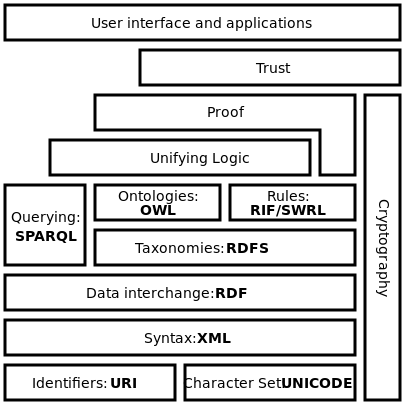
\includegraphics[width=.40\textwidth]{semantic_web_stack} 
%  \caption{Camadas da Web Semântica}
%  \label{fig:arquitetura_web_semantica} 
%\end{figure}

\section{\emph{Ontologias}}
\label{sec:ontologias}

A ontologia é uma palavra que deriva do grego "onto" de ser e "logia" representado o discurso escrito ou falado tendo suas suas raízes no campo da Filosofia com estudo de teorias da natureza da existência \citet{Berners-lee2001}. De posse desse significado, pesquisadores da web de dados, da inteligência artificial, entre outros, passaram a adotar o termo para definir conceitos de maneiras que eles possam ser processados pelas máquinas. Conceitos esses que podem ser taxonomias, assim como ilustra a imagem \ref{fig:exemplo_taxonomia}, classificações ou outras formas de representar domínios de conhecimento, geralmente visando o compartilhamento e reúso de dados.

\begin{figure}[!ht]
  \centering
  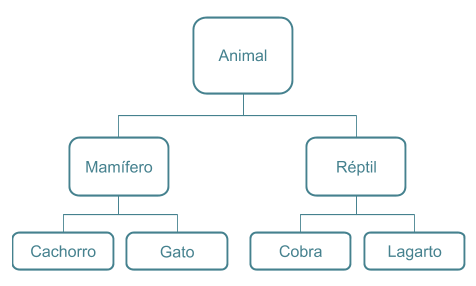
\includegraphics[width=.95\textwidth]{exemplo_taxonomia} 
  \caption{Exemplo de taxonomia}
  \label{fig:exemplo_taxonomia} 
\end{figure}

Ontologia são o coração da Web Semântica. São elas que formalizam o conhecimento sobre um domínio especifico de maneira a tornar possível a interpretação do significado de dados contidos em diferentes documento pelos computadores \citep{Bienvenu2013} e possibilitam um processamento automatizado e mais eficiente da informação. Em outras palavras, pode ser entendida como a especificação explícita de uma conceitualização \citep{Gruber1993} consistindo de diversos conceitos a respeito de um contexto que são expressados em uma linguagem que possui semântica bem definida, de fácil compreensão e leitura \citep{Gali2004}. É a descrição formal explícita de conceitos que podem ser descritos como classes formadas por atributos que descrevem características e por restrições \citep{Jain2011}.

O problema da unificação de diferentes formas de dados pode ser superado por meio da exploração semântica com o uso de ontologias. Por serem caracterizadas por diversos conceitos a respeito de um domínio e serem expressas em uma linguagem que possui semântica bem definida, de fácil compreensão e leitura \citep{Gali2004, Kabir2014} acabam promovendo um entendimento único e compartilhado dos dados que existem dentro de um determinado domínio de integração. Desse modo, um dos objetivos mais comuns para o desenvolvimento de ontologias é o de compartilhar o entendimento comum da estrutura da informação \citep{Noy2001}. Assim, a Web semântica aproxima a possibilidade de realização de repositórios com dados organizados que podem ser utilizados para a pesquisa de informação inteligente para humanos e agentes computacionais \citep{Gali2004} na Internet.





Regras de inferências nas ontologias adicionam ainda mais poder. Uma ontologia pode expressar uma regras para que o programa possa deduzir coisas como Se A USP está em Sâo Paulo e são paulo e uma cidade do brasil, então a usp está no brasil.

A ontologias podem melhorar a funcionalidade da Web. Podem auxiliar a melhorar a 
acurácia de buscadores por buscas acerca de um conceito sem abiguidade.


\section{\emph{Projetos de definição de ontologias}}
\label{sec:projetos_de_ontologias}

Em meio a necessidade de definição de ontologias visando a padronização dos conceitos acerca de domínios e com o objetivo de possibilitar o entendimento dos dados pelas máquinas e assim alcançar a integração de dados na internet, diversos esforços surgiram por parte da comunidade cientifica e por iniciativas privadas. Entre os projetos mais importantes podemos citar o Schema.org, o vocabulário FOAF, o DBPedia e o Linking Open Data.

\subsection{\emph{A iniciativa Schema.org}}
\label{sec:iniciativa_schema_org}

Interessados pela possibilidade de entregar conteúdo mais relevante e personalizado para seus usuários, os maiores portais de de pesquisa de dados a época, Google, Bing, Yahoo e o Yandex\footnote{\url{http://www.yandex.com/}} criaram a iniciativa Schema.org\footnote{\url{http://schema.org/}}. A ideia por trás desse esforço conjunto se traduz em melhorar a acurácia e apresentação de resultados da pesquisa nesses portais por meio da criação de marcações padronizadas que podem ser adicionadas pelos desenvolvedores das páginas HTML fazendo com que a máquina possa interpretar melhor os dados ali contidos \citep{Tort2014, Mika2015}. Desse modo, o portal Schema.org se estabeleceu com um conjunto padronizado de de ontologias, construídas a partir de esforços já pré-existentes para a criação de terminologias, que estão sendo cada vez mais adotadas em larga escala \citep{Mika2015}.

Conforme \citet{Mika2015}, o portal Schema.org prove é portal centralizado de ontologias constituído pela documentação e exemplos de uso de classes que representam os tipos de dados mais populares contidos na Web como a representação do perfil de uma pessoa, informações sobre produtos, entidades de negócio, eventos, organizações, entre outros. A Figura~\ref{fig:exemplo_organizacao_schema_org} representa um exemplo de documentação no portal\footnote{\url{http://1.schemaorgae.appspot.com/Organization}}. Nesse exemplo podemos notar a descrição de uma organização (Organization), a quantidade de uso dessa classe em diferentes portais da Web, todas as propriedades dela como o endereço (\emph{"address"}), email, entre outros, o tipo de cada uma dessas propriedades e a descrição do que é cada uma delas.

\begin{figure}[!ht]
  \centering
  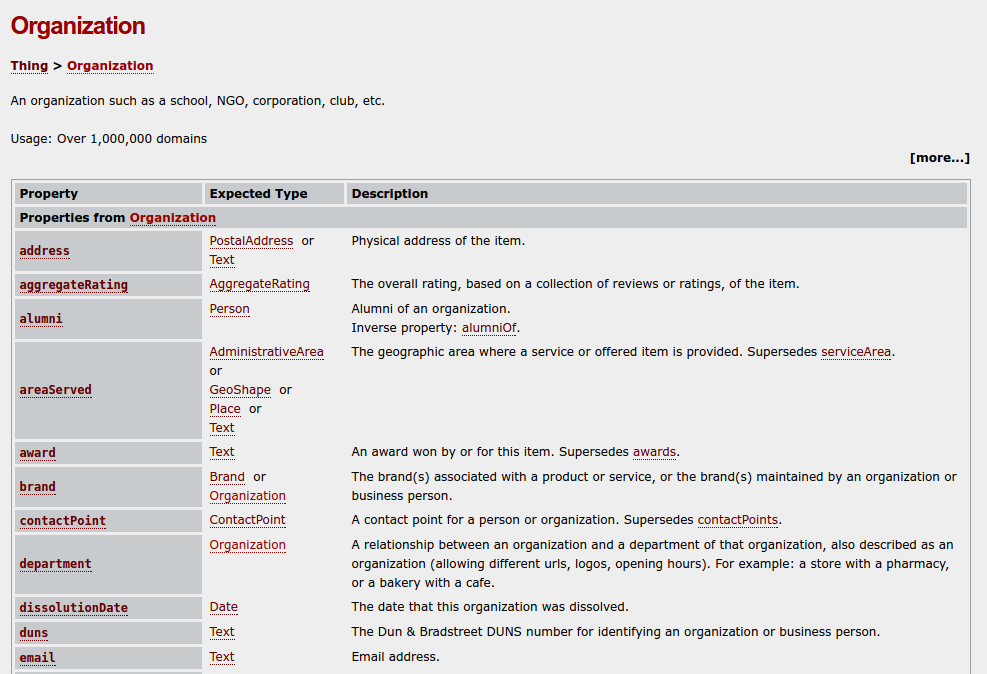
\includegraphics[width=.95\textwidth]{exemplo_organizacao_schema_org} 
  \caption{Exemplo da definição de uma organização pelo projeto Schema.org}
  \label{fig:exemplo_organizacao_schema_org} 
\end{figure}

\subsection{\emph{Os projetos DBpedia e Linking Open Data}}
\label{sec:projeto_dbpedia}

O Wikipédia\footnote{\url{https://www.wikipedia.org/}} é hoje a enciclopédia digital e um dos portais mais importante do planeta contando com informações nas mais diversas linguagens. Nele é disponibilizado o esforço de uma produção colaborativa de pessoas que produzem o conteúdo e que o revisam para garantir boa qualidade dos dados ali apresentados.No entanto, a informação ali contida está limitada a busca por palavras chaves e isso gera uma série de problemas que vão desde dados contraditórios, inconsistência de convenções taxonômicas, erros ou até spam \citep{Auer2007}. Levando isso em consideração, o DBpedia foi criado com o objetivo de colocar uma camada semântica sobre o conteúdo ali exposto e, com isso, solucionar parte dos problemas colocados a partir de consultas mais sofisticadas.

O projeto DBpedia é um esforço de extração dos dados da Wikipédia e conversão para documentos de formato RDF. De acordo com \citet{Auer2007} é um trabalho que hoje conta com muitos milhões de triplas RDF e que se interliga com outras bases de informação, conforme representado na Figura~\ref{fig:dbpedia_interligacao_dados}, podendo ser expandido para um conjunto de bilhões de triplas. Toda os dados extraídos são expostos para consultas na internet a partir de uma infra-estrutura refinada que conta com bancos relacionais MySQL e bancos de consulta com anotações semânticas do do tipo Virtuoso\footnote{\url{https://virtuoso.openlinksw.com/}}. Esse esforço faz parte da comunidade que mantém o projeto Linking Open Data\footnote{\url{http://linkeddata.org/}} (LOD) que tem o interesse de criar uma grande quantidade de conjunto de dados e ontologias interligado, contribuindo com a Web Semântica e que em agosto de 2014 já assimilava quase 600 conjuntos de dados além do DBPedia conforme ilustra a Figura~\ref{fig:lod_graph_agosto_2014}. 

\begin{figure}[!ht]
  \centering
  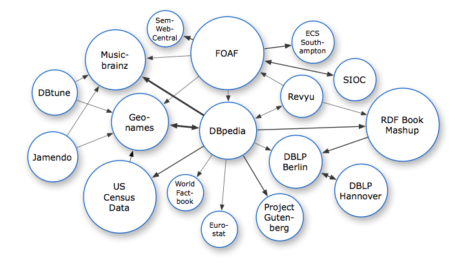
\includegraphics[width=.95\textwidth]{dbpedia_interligacao_dados} 
  \caption{Integração de dados no DBpedia \citep{Auer2007}}
  \label{fig:dbpedia_interligacao_dados} 
\end{figure}

\begin{figure}[p]
  \centering
  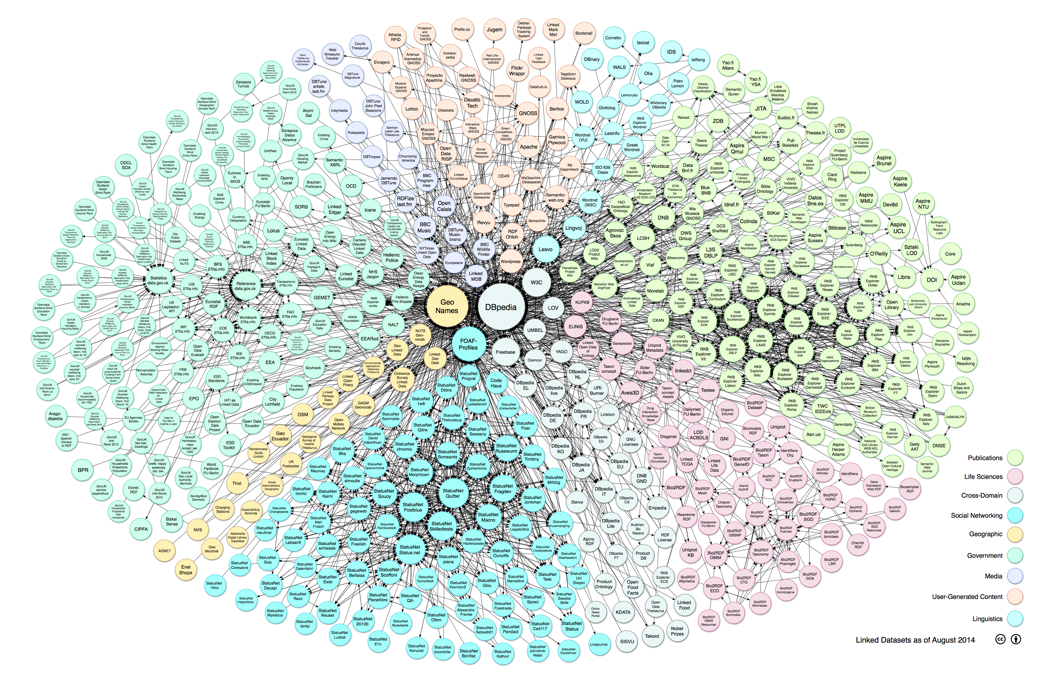
\includegraphics[angle=90, scale=0.65]{lod_graph_agosto_2014} 
  \caption{Integração de fontes de dados abertos em agosto de 2014 \citep{Cyganiak2014}}
  \label{fig:lod_graph_agosto_2014} 
\end{figure}

\section{\emph{Linguagens da Web Semântica}}
\label{sec:linguagens_web_semantica}

De acordo com \citet{Allemang2011}, as tecnologias necessárias para habilitar essa nova Web já estão disponíveis: a linguagem de marcação XML (\emph{Extensible Markup Language}), a linguagem HTML (\emph{HyperText Markup Language}) e o Framework de descrição de recursos RDF (\emph{Resource Description Framework}), uma linguagem de descrição geral para descrição de ontologias \citep{Wang}. Além disso, em conjunto com o protocolo SPARQL para consulta em RDF (\emph{SPARQL query language for RDF}), tornam possível a integração de dados provenientes de diferentes base de dados, documentos, motores de inferência ou qualquer outra fonte de informação que possa expressar conhecimento \citep{Wang}.

\subsection{\emph{HyperText Markup Language} (HTML)}
\label{sec:html}

Uma parcela considerável da informação publicada mundialmente na internet é estabelecida através de documentos no formato HTML. Isso porque essa linguagem foi projetada para estruturar a informação de maneira tal que um navegador possa interpretar a estrutura dos dados ali definida e exibi-la com botões, textos, entre outros elementos para que um usuário possa entende-la. Além disso, como é baseada em um padrão de marcação de dados estabelecido pela norma ISO8879 que define o SGML (\emph{Standard Generalized Markup Language}) possui tags específicas que lembram um documento XML mas tem por responsabilidade representar os diversos elementos de uma página conforme ilustra a Imagem~\ref{fig:exemplo_codigo_html}.



%\citep{Wilde2008} Even though it focuses on human-readable documents, HTML has mechanisms for link semantics, most notably the link element in the document head. HTML itself defines a number of possible relations to associated resources, and some of these are also used in a more de-facto standard way to detect certain common resource types.2 HTML also de- fines structural links between Web resources, though few Web sites and browsers expose this information natively. This is still a very simplistic linking model, expressing a one-way linkage between a given resource and some con- textual resource or association. Link information is exclu- sively controlled by the author or publisher of the HTML document, and is bound to the specific document that con- tains it.


\begin{figure}[!ht]
    \begin{lstlisting}[language=HTML,frame=trbl]
<!DOCTYPE html>
<html>
<head>
  <title>Titulo da pagina</title>
</head>
<body>

  <h1>Cabecalho</h1>
  <p>Paragrafo.</p>
  
</body>
</html>
    \end{lstlisting}
    \caption{Exemplo de código HTML}
    \label{fig:exemplo_codigo_html} 
\end{figure}

\subsection{\emph{eXtended Markup Language} (XML)}
\label{sec:xml}

%\citep{Berendt2004}
%Beside annotation for for- matting, XML allows the definition of any kind of annotation, thus opening the way to annotation with ontologies and to use as data model for arbitrary information. This makes it extensible, unlike its ancestors like HTML

Em virtude da publicação de informação em larga escala nos meios eletrônicos tornou-se necessário a existência de um mecanismo capaz de facilitar a troca de uma grande variedade de dados \citep{W3C_XML}. Nesse contexto, o XML surge com o objetivo de descrever uma classe de objetos voltados para marcação dos dados em documentos diferentemente do HTML que foi projetado para marcação de estruturade exibição em navegadores. Exemplos da versatilidade da aplicação do XML vão desde páginas na internet, livros, interfaces de programação ou a representação bancos de dados relacionais e seu conteúdo permitindo inclusive o processamento de dados que não estavam previamente armazenados como XML \citep{Wang}. Além disso, a manipulação de um documento XML é feita de maneira trivial pela grande maioria das linguagens de programação \citep{Heath2008},
 
O documento XML consiste em unidades de armazenamento chamadas de entidades e que formam, em conjunto, uma árvore de nós ordenados. Essas entidades, formadas por caracteres, delimitam os dados através de marcações formando assim o modelo de armazenamento da informação e a estrutura lógica do documento. Além disso, a ordem entre as entidades é relevante, a ponto de que a alteração entre elas pode fazer com que o documento não possa ser devidamente interpretado por ferramentas de software. Dessa maneira, permite-se a criação de rótulos, assim como ilustrado pela Figura~\ref{fig:exemplo_codigo_xml} como <cep> ou <nome> que podem ser interpretados a partir da implementação de programas. 

\begin{figure}[!ht]
    \begin{lstlisting}[language=XML]
<?xml version="1.0" encoding="UTF-8"?>
<pessoa>
	<nome>Felipe</nome>
	<sobrenome>Pierin</sobrenome>
	<email>fpierin@ime.usp.br</email>
	<geolocalizacao latitude="-23.558745" longitude="-46.731859" />
	<endereco>
		<cep>05508-090</cep>
		<cidade>Sao Paulo</cidade>
	    <rua>Rua do Matao, 1010</rua>
	</endereco>
</pessoa>	
    \end{lstlisting}
    \caption{Exemplo de um documento XML}
    \label{fig:exemplo_codigo_xml} 
\end{figure}

O documento XML conciso respeita alguma condições simples como é possível verificar a partir exemplo de documento XML proposto na Figura~\ref{fig:exemplo_codigo_xml}. A primeira condição é que toda marcação tem seu inicio e fim. Isso significa que um rótulo do tipo "<nome>" obrigatoriamente tem seu contraponto "</nome>" a menos que ele seja auto-contido como o exemplo da "geolocalizacao" na linha 6. Além disso o documento está contido em uma única marcação e todas elas estão aninhadas. A linha 7, por exemplo, mostra uma tag que contém outras tags filhas. No entanto, como essas estruturas não possuem semântica sobre o significado, faz-se necessário o entendimento da estrutura por parte do projetista do sistema \citep{Allemang2011}.

%\begin{figure}[!ht]
%  \centering
%  \fbox{%
%    \begin{minipage}{\dimexpr.60\textwidth-1\fboxsep-1\fboxrule}\centering
%    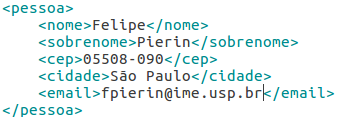
\includegraphics[width=.99\textwidth]{exemplo_codigo_xml} 
%    \end{minipage}
%  }
%  \caption{Exemplo de um documento XML}
%  \label{fig:exemplo_codigo_xml} 
%\end{figure}

%\citep{Quboa2013}
%precisely answer and satisfy the web users’ requests [1,5, 6]. Semantic Web is a part of the second generation web (Web2.0) and its original idea derived from the vision W3C’s director and the WWW founder, Sir Tim Berners- Lee. According to [5] Semantic Web represents the ex- tension of the World Wide Web that gives users of Web the ability to share their data beyond all the hidden barri- ers and the limitation of programs and websites using the meaning of the web.
%2.2. Reasons behind Developing Semantic Web
%As noted by [7], the Semantic Web is introduced to crack two specific problems: the limitations of data access in the web (for example retrieving documents according to a given request using ambiguous terms, and the current retrieving systems problem of acquiring only a single “best fit” documents for a query), and the delegation tasks’ problems (such as integrating information) by sup- porting access to data at web-scale and enabling the de- legation of certain classes of tasks.
%2.3. Semantic Web Representation Techniques
%Many available techniques and models are used to repre- sent and express the semantic of data such as the stan- dard techniques recommended by W3C named Extensi- ble Markup Language, Resource Description Framework, and Web Ontology Language [5] which are briefly ex- plained below.
%2.3.1. Extensible Markup Language The Extensible Markup Language (XML) technique has been established as a generic technique to store, organize, and retrieve data on/from the web. By enabling users to create their own tags, it allows them to define their con- tent easily. Therefore, the data and its semantic relation- ships can be represented

%\citep{Stumme2006}
%XML and XML schema were designed to describe the struc- ture of text documents, like HTML,Word, StarOffice, or L
%ATEX
%documents. It is possible to define tags inXMLto carry metadata but these tags do not have formally defined semantics and thus their meaning will not be well-defined. It is also difficult to con- vert oneXMLdocument to another one without any additionally specified semantics of the used tags. The purpose of XML is to group the objects of content, but not to describe the content. Thus,XMLhelps the organization of documents by providing a formal syntax. This is not ‘semantic’ in the sense of our survey. Erdmann [48] provides a detailed analysis of the capabilities of XML, the shortcomings of XML concerning semantics, and possible solutions.

\subsection{\emph{Resource Description Framework} (RDF)}
\label{sec:rdf}

Na Web Semântica todas as coisas são definidas como recursos, sejam relacionamento entre entidades ou ela própria \citep {Allemang2011}. Nesse sentido, o RDF é uma recomendação da W3C para padronizar o uso de descrições de metadados de recursos baseados na WEB \citep{VanDeursen2008} para representar, entre outras coisas, informações pessoais, redes sociais, metadados de artefatos digitais e promover meios de integrar fontes diferentes de informação visando facilitar a troca, fusão e compartilhamento de dados por aplicações diversas. Iniciativas como o DBPedia \footnote{\url{http://wiki.dbpedia.org/}}, o projeto \emph{Linked Open Data}\footnote{\url{http://linkeddata.org/}} e o projeto Schema.org\footnote{\url{http://schema.org/}} estão tranformando a Web Semântica auxiliando na tranfosrmação dos dados para RDF e permitindo assim a interligação entre as diversas fontes existentes \citep{Heath2008}.

O RDF é uma extensão do mecanismo de \emph{hyperlinks} e faz a conexão entre recursos da Web atual usando os identificadores de recursos chamados URI (\emph{Uniform Resource Identifier}) para definir não só relacionamento entre coisas mas também os dois extremos dessa conexão. Desse modo, conforme exemplificado pela figura~\ref{fig:estrutura_triplas_rdf}, a estrutura básica de um documento RDF possui três elementos chaves: o sujeito, um predicado e o objeto de referência. O sujeito ao qual estabeleceremos atributos como, por exemplo, uma pessoa, um automóvel ou uma faculdade, uma entidade objeto que define algum valor tal qual um nome, uma cor ou uma matéria, e um predicado que estabelece a relação entre esse sujeito e o valor como, por exemplo, "conhece", "é amigo de", "é filho de". No exemplo anterior é possível observar que o sujeito é "Felipe Pierin", representado pelo URI "\url{http://www.example.org/persons/Felipe_Pierin}", o predicado "mora\_em" (\url{http://www.example.org/properties/mora_em}) e o objeto "São Paulo" (\url{http://www.example.org/places/Sao_Paulo}).

\begin{figure}[!ht]
  \centering
  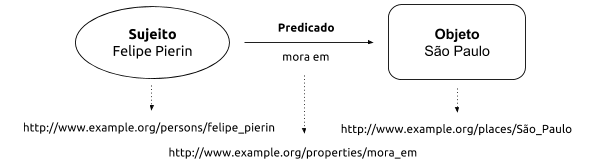
\includegraphics[width=.70\textwidth]{estrutura_triplas_rdf} 
  \caption{Estrutura básica de uma tripla RDF}
  \label{fig:estrutura_triplas_rdf} 
\end{figure}

Ao expandir esse simples modelo para inúmeras conexões, alcançamos uma rede de recursos de informações, inter-relacionados por propriedades que estabelecem uma relação entre essas triplas e que formam um grafo RDF conforme exemplificado pela imagem imagem~\ref{fig:grafo_rdf}. Essa é uma característica importante pois permite que a informação seja misturada com facilidade uma vez que faze-lo depende apenas da junção dos diferentes grafos de interesse uma vez que é acaba por ser a maneira natural de descrever uma parcela considerável dos dados processados por máquinas \citep{Allemang2011}. Além disso, como a publicação e conversão de documentos em RDF adiciona semântica ao recursos, ela também promove a integração da informação na internet proveniente de fontes de dados diversas uma vez que unifica o entendimento a respeito de um conteúdo, permite um melhor entendimento das máquinas a respeito de um determinado domínio e ainda e torna possível a busca de conteúdo relevante por meio de linguagem padrão de consulta, o SPARQL \citep{Heath2008}.

\begin{figure}[!ht]
  \centering
  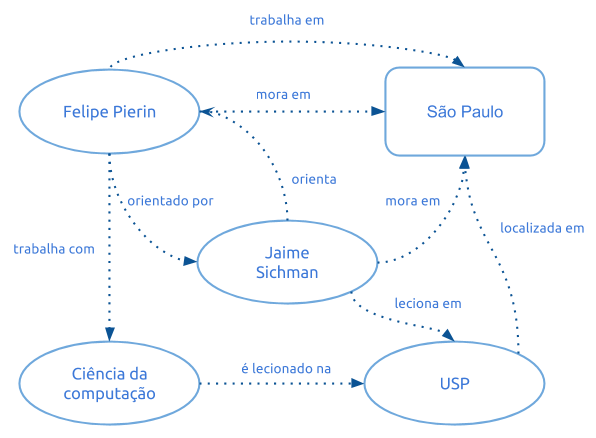
\includegraphics[width=.95\textwidth]{grafo_rdf} 
  \caption{Exemplo de grafo RDF}
  \label{fig:grafo_rdf} 
\end{figure}

Por fim, outra propriedade relevante de um documento RDF é que ele pode ser representado em uma estrutura XML assim como ilustrado pela figura~\ref{fig:exemplo_codigo_rdf}. Nesse exemplo há a definição de um objeto do tipo "Person" e que possui um nome definido na marcação "name" e um email definido por "mbox". Essa forma de apresentação é denominada RDF/XML e têm sido amplamente utilizadas para retratar informações semanticamente anotadas.

%\begin{figure}[!ht]
%  \centering
%  \fbox{%
%    \begin{minipage}{\dimexpr.95\textwidth-1\fboxsep-1\fboxrule}\centering
%    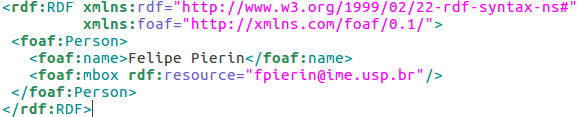
\includegraphics[width=.99\textwidth]{exemplo_codigo_rdf} 
%    \end{minipage}
%  }
%  \caption{Exemplo de um documento RDF em XML}
%  \label{fig:exemplo_codigo_rdf} 
%\end{figure}

\begin{figure}[!ht]
    \begin{lstlisting}[language=XML]
<rdf:RDF xmlns:rdf="http://www.w3.org/1999/02/22-rdf-syntax-ns#"
         xmlns:foaf="http://xmlns.com/foaf/0.1/">
 <foaf:Person>
   <foaf:name>Felipe Pierin</foaf:name>
   <foaf:mbox rdf:resource="fpierin@ime.usp.br"/>
 </foaf:Person>
</rdf:RDF>
    \end{lstlisting}
    \caption{Exemplo de um documento RDF em XML}
    \label{fig:exemplo_codigo_rdf} 
\end{figure}

\subsection{\emph{SPARQL Protocol and RDF Query Language} (SPARQL)}
\label{sec:sparql}

Em virtude do documento RDF poder ser entendido como um grafo direcionado para a representação de informação, iniciativas como o SPARQL nasceram para aproveitar essa característica. O protocolo de busca em RDF é, de maneira simplificada, uma linguagem de consulta de correspondência em Grafos. Desse modo, levando em consideração uma fonte de dados em RDF, a consulta seria um padrão combinado contra essa fonte e os valores obtidos a partir dessa correspondência são processados para dar a resposta \citep{Perez2006}. Além disso, uma consulta SPARQL não precisa ser restrita a uma única fonte de informação (\emph{endpoint} SPARQL), isso é, vários grafos RDF podem ser combinados dentro de uma única pesquisa. Sejam eles documentos RDF nativos ou gerados em tempo de execução via outros sistemas intermediários \citep{W3C_SPARQL}. Por esse motivo, essa linguagem é fundamental no que diz respeito ao Linked Data pois é ela que permite a extração de conhecimento dos diversos endpoints SPARQLs distribuídos \citep{Singh2010}.

Conforme observado por \citet{Perez2006}, uma consulta SPARQL apresenta três partes fundamentais: a correspondência de padrões, os modificadores de resultado e o resultado final. O exemplo de um código SPARQL é ilustrado pela Figura~\ref{fig:exemplo_codigo_sparql} .No que diz respeito a correspondência de padrões, a linguagem não só apresenta características de correspondência de padrões em gráficos tal qual partes opcionais, união, aninhamento e filtragem como também permite restringir à qual fonte de dados será aplicada. Já os modificadores de resultado permitem modificar os valores encontrados uma vez que a saída padrão já foi computada. Por fim, o resultado final pode ser tanto um valor específico como sim ou não ou mesmo uma sub-grafo das fontes iniciais utilizadas na consulta.

%\begin{figure}[!ht]
%  \centering
%  \fbox{%
%    \begin{minipage}{\dimexpr.65\textwidth-1\fboxsep-1\fboxrule}\centering
%    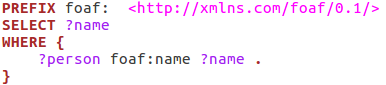
\includegraphics[width=.99\textwidth]{exemplo_codigo_sparql} 
%    \end{minipage}
%  }
%  \caption{Exemplo de consulta SPARQL}
%  \label{fig:exemplo_codigo_sparql}
%\end{figure}

\begin{figure}[!ht]
    \begin{lstlisting}[language=SPARQL]
PREFIX foaf:  <http://xmlns.com/foaf/0.1/>
SELECT ?name
WHERE {
    ?person foaf:name ?name .
}
    \end{lstlisting}
    \caption{Exemplo de consulta SPARQL}
    \label{fig:exemplo_codigo_sparql} 
\end{figure}

% A type may be an object type or a property2. Each type has a name and a description. An object type may be an entity type, a data type or an enumeration. An enumeration consists of a set of literals. A property may have one or more entity types as its domain and one or more object types as its range. For example, the property creator has as its domain CreativeWork and UserComments, and its range may be an Organization or a Person.

%Types are arranged in a multiple specialization/generalization hierarchy where each type may be a subtype of multiple supertypes. For example, the entity type LocalBusiness is a subtype of both Organization and Place. The top of the hierarchy is the entity type Thing. All other object types are a direct or indirect subtype of it. A property may also be a subtype of another one, although this is used only in user extensions to schema.org. Enumerations may have subtypes. For example, MedicalSpecialty is a subtype of Specialty.







%LOD data can be either dumped or accessed via SPARQL endpoints which are web services enabling users to query a knowledge base via the SPARQL language. Using


%\citep{Quilitz2008}
%Before we describe our work on federated queries we give a short introduction to the SPARQL query language and the operators of a SPARQL query that are considered for this report. For a more detailed %introduction to RDF and SPARQL we refer the interested reader to [14, 1, 15]. In the following we use the definitions from the SPARQL Recommendation in [1]. A SPARQL query Q is defined as tuple Q = (E,DS,R). %Basis of SPARQL
%query is an algebra expression E that is evaluated with respect to a RDF graph in a dataset DS. The results of the matching process are processed according to the definitions of the result form R (SELECT, %CONSTRUCT, DESCRIBE, ASK). The algebra expression E is build from different graph patterns and can also also include solution modifiers, such as PROJECTON, DISTINCT, LIMIT, or ORDER BY. The simplest graph %pattern defined for SPARQL is the triple pattern. A triple
%pattern t is similar to a RDF triple but allows the usage of variables for subject, predicate, and object:
%t ∈ TP = (RDF-T ∪ V )×(I ∪ V )×(RDF-T ∪ V )
%with RDF-T being the set of RDF Terms (RDF Literals and Blank Nodes), I being a set of all IRIs, and V a set of all variables [1].

%\citep{Wang}
%The SPARQL query language is based on matching graph patterns. Graph patterns contain triple patterns that are like RDF triples, but with the option of query va- riables in place of RDF terms in the subject, predicate or object positions. Combining triple patterns gives a basic graph pattern, more complex graph patterns can be formed by combining smaller patterns. The triple patterns of a SPARQL query over domain ontology can be considered as a sub-graph of the RDF Graph.




%\section{\emph{Ontologias}}
%\label{sec:ontologias}




%\citep{VanDeursen2008} A utilização de RDF e outras tecnologias SemanticWeb baseadas no RDF, como o RDF Schema (RDFS,[3]) e o Web Ontology Language (OWL, [15]), podem resolver o problema de interoperabilidade semantica. Assim, ao invés de anXML Schema, é criada uma ontologia, que é um modelo de dados representando um conjunto de conceitos dentro de um domínio, juntamente com as relações entre esses conceitos. No entanto, como a maioria dos metadados está disponível em formato XML, as ontologias estão sendo feitas com base nas normas de metadados existentes. A partir de um XML Schema, muitos esforços estão sendo feitos para criar uma ontologia OWL. Exemplos de tais padrões para os quais as representações semânticas foram criadas são MPEG-7 [11], DIG351 e Exif2

%\citep{Stumme2006}
%The Semantic Web is based on a vision of Tim Berners-Lee, the inventor of the WWW

%\citep{Stumme2006}
%1. Providing a common syntax for machine understandable statements.
%2. Establishing common vocabularies. 
%3. Agreeing on a logical language. 
%4. Using the language for exchanging proofs.

%\citep{Stumme2006}
%Berners-Lee suggested a layer structure for the Semantic
%Web. This structure reflects the steps listed above. It follows the understanding that each step alone will already provide added value, so that the SemanticWeb can be realized in an incremental fashion.
%2.1. Layers of the Semantic Web Figure 1 shows the layers of the SemanticWeb as suggested
%by Berners-Lee.2 This architecture is discussed in detail for in- stance in [126] and [127], which also address recent research questions. Onthe firsttwolayers, acommonsyntax is provided. Uniformresource identifiers (URIs) provide a standard way to refer to entities,3 while Unicode is a standard for exchanging symbols. The Extensible Markup Language (XML) fixes a notation for describing labeled trees, andXMLSchema allows the definition of grammars for valid XML documents. XML documents can refer to different namespaces to make explicit the context (and therefore meaning) of different tags. The formalizations on these 2